\chapter[Otimização multiobjetivo]{Otimização multiobjetivo}

A otimização multiobjetivo consiste em selecionar as melhores soluções de acordo com múltiplos critérios ao invés de apenas um. Por exemplo, ao estabelecer um melhor caminho entre duas cidades pode-se não estar interessado apenas na menor distância, mas também no tráfego, segurança das vias, quantidade de pedágios, etc. A otimização de apenas um objetivo é simples, para que uma solução seja considerada melhor que a outra, basta que ela tenha uma melhor avaliação. Por outro lado, quando se trabalha com mais de uma função de otimização, é preciso usar o conceito de dominância de Pareto.

A dominância de Pareto diz que uma solução $A$ é melhor que uma solução $B$, ou $A$ domina $B$ ($A \prec B$), se, e somente se:

\begin{itemize}  
	\item $A$ é melhor avaliado que $B$ em pelo menos um dos objetivos;
	\item $A$ não tem avaliação pior que $B$ em nenhum dos objetivos.
\end{itemize}

Considerando um problema de minimização e $F$ como o conjunto de funções objetivo, tem-se, matematicamente:

\[A \prec B \Leftrightarrow (\forall(f \in F) f(A) \leq f(B)) \land (\exists (f \in F) f(A) < f(B))\]

Em problemas de otimização multiobjetivo, o interesse está em encontrar o conjunto de todas as soluções que não são dominadas por nenhuma outra, ou seja, a fronteira de Pareto. Graficamente, a fronteira de Pareto representa a linha formada pelas soluções não-dominadas existentes para o problema. Na figura \ref{fig_pareto} apresenta-se um exemplo de uma fronteira de Pareto para um problema de minimização com dois objetivos ($F1$ e $F2$), a fronteira de Pareto está representada em vermelho. Observe que nenhum círculo vermelho possui ambos F1 e F2 menores que alguma outra solução em vermelho, ou seja, são não-dominadas. Em contra-partida, toda solução acima da fronteira, em cinza, é dominada, pois existe alguma solução em vermelho que possui ambos valores de F1 e F2 menores. Caso o problema em questão fosse de maximização, a fronteira de Pareto estaria acima de qualquer solução não-dominada ao invés de abaixo.

\begin{figure}
	\label{fig_pareto}
	\caption{Fronteira de Pareto}
	\centering
	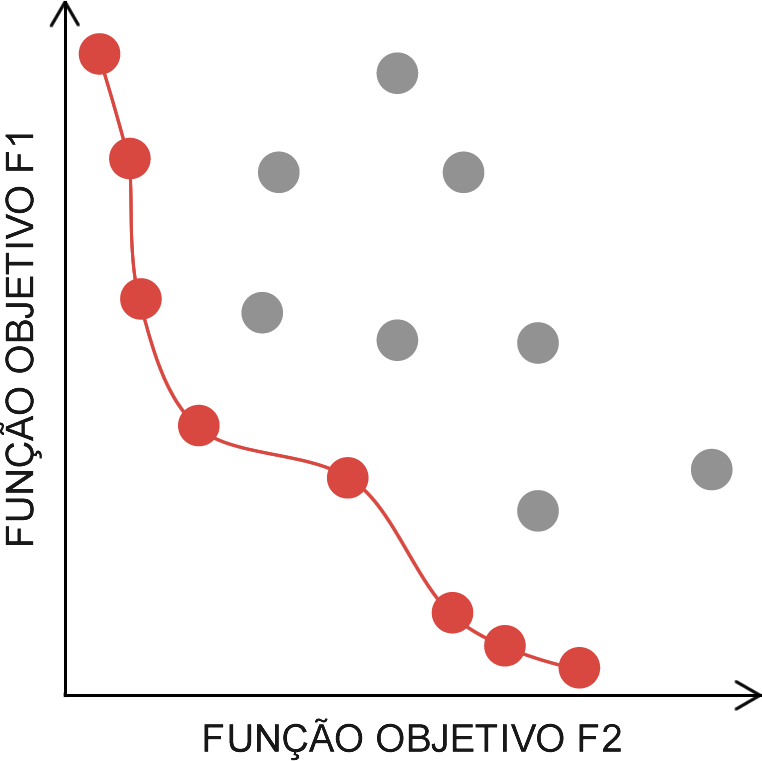
\includegraphics[width=0.4\textwidth]{cap_otimizacao-multi/figs/pareto}
\end{figure}

Não existe limite para o número de funções objetivo em um problema de otimização, mas quanto maior ele for, mais complexa é a busca. Os algoritmos clássicos de otimização multiobjetivo NSGA-II e SPEA2 lidam bem com até dois objetivos, mas a partir de quatro critério de otimização, ambos os métodos sofrem para encontrar soluções relevantes. Desta forma, criou-se a classificação "many-objective". Problemas many-objectives (4 ou mais objetivos) apresentam diversas novas dificuldades e precisam de novas técnicas para que sejam resolvidos eficientemente. Como observado por Deb em [nsga3], os problemas trazidos pelo alto número de objetivos são:

\begin{enumerate}  
	\item Grande parte da população é não dominada: a maioria dos algoritmos multiobjetivos classifica a população de acordo com a dominação de Pareto. Se existem muitas funções objetivo, se torna muito comum que uma solução seja melhor que outra em pelo menos uma das funções. Desta forma, a maior parte das soluções se torna não-dominada, o que impede os algoritmos de evoluírem a população, já que todos os indivíduos são considerados igualmente bons.
	\item Avaliar a diversidade da população se torna computacionalmente caro: afim de garantir uma boa diversidade populacional, alguns algoritmos medem alguma espécie de distância entre as soluções e removem as que são consideradas mais similares. A maior dimensionalidade traz consequentemente um maior impacto no cálculo da proximidade entre os indivíduos. 
	\item Crossover ineficiente: a alta dimensionalidade do espaço de busca faz com que os indivíduos na população sejam muito distante uns dos outros e, normalmente, o cruzamento entre duas soluções muito diferentes resultam num filho muito distante dos pais, o que prejudica a convergência da busca. Portanto, pode ser necessário redefinir os operadores de recombinação afim de restringir as possibilidades de pareamento.
	\item 
	\item 
	\item 
\end{enumerate}